\documentclass[tikz,border=5pt]{standalone}
\usepackage{tikz}
\usetikzlibrary{arrows.meta}
\definecolor{nebula}{HTML}{6366F1}
\definecolor{spark}{HTML}{14B8A6}
\definecolor{ink}{HTML}{334155}
\begin{document}
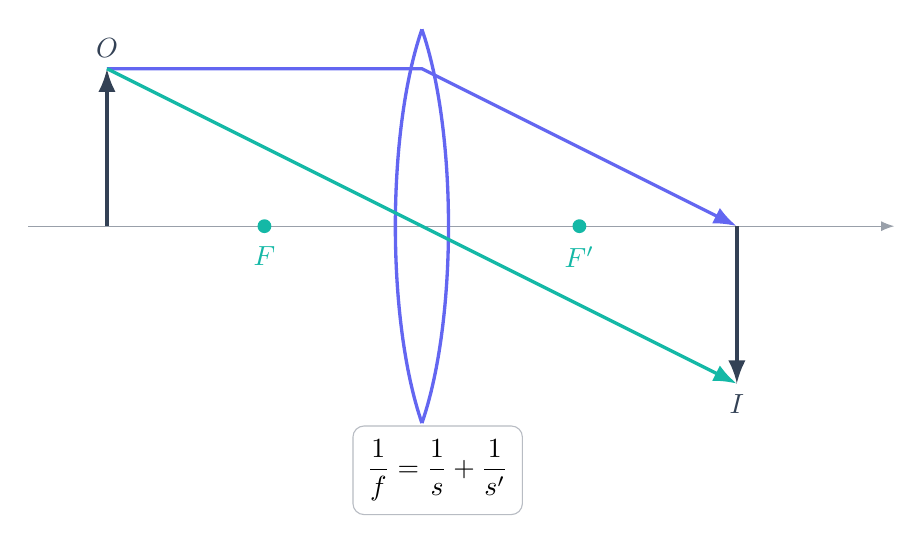
\begin{tikzpicture}[x=1cm,y=1cm,font=\sffamily,>=Latex]
  \draw[->,ink!50] (-5,0)--(6,0);
  \draw[very thick,nebula] (0,-2.5)..controls(-.45,-1.2)and(-.45,1.2)..(0,2.5);
  \draw[very thick,nebula] (0,-2.5)..controls(.45,-1.2)and(.45,1.2)..(0,2.5);
  \fill[spark] (-2,0) circle (2.5pt) node[below=4pt] {$F$};
  \fill[spark] (2,0) circle (2.5pt) node[below=4pt] {$F'$};
  \draw[very thick,ink,->] (-4,0)--(-4,2) node[above] {$O$};
  \draw[very thick,nebula,->] (-4,2)--(0,2)--(4,0);
  \draw[very thick,spark,->] (-4,2)--(0,0)--(4,-2);
  \draw[dashed,ink!35] (4,-2)--(4,0);
  \draw[very thick,ink,->] (4,0)--(4,-2) node[below] {$I$};
  \node[draw=ink!35,rounded corners=4pt,fill=white,inner sep=5pt] at (.2,-3.1) {$\displaystyle\frac1f=\frac1{s}+\frac1{s'}$};
\end{tikzpicture}
\end{document}
